\documentclass{article}

%
% 引入模板的style文件
%
\usepackage{homework}

\setCJKmainfont{SimSun}[AutoFakeBold] %宋体加粗
\setCJKsansfont{SimHei}[AutoFakeBold] %黑体加粗


\usepackage{minted} %配合minted宏包进行好看的高亮
\usepackage{currfile} %配合minted宏包进行好看的高亮
\usepackage{caption} %配合minted宏包进行好看的高亮
\usepackage{tcolorbox} %配合minted宏包进行好看的高亮
\usepackage{xcolor} %配合minted宏包进行好看的高亮
\tcbuselibrary{skins} %配合minted宏包进行好看的高亮
\tcbuselibrary{minted} %配合minted宏包进行好看的高亮
\usemintedstyle{paraiso-dark} %配合minted宏包进行好看的高亮



%
% 封面
%


\title{
	
\includegraphics[width=0.6\textwidth]{images/title/ucas_logo 1.pdf}\\
    \vspace{1in}
    \textmd{\textbf{\hmwkClass}}\\
	\textmd{\Large{\textbf{\hmwkClassID}}}\\
    \textmd{\textbf{\hmwkTitle}}\\
    \normalsize\vspace{0.1in}\large{\hmwkCompleteTime }\\
    \vspace{0.1in}\large{\textit{\hmwkClassInstructor\ }}\\
    \vspace{1in}
	
\includegraphics[width=0.25\textwidth]{images/title/Cyber.jpg}\\
	\vspace{1in}
}

\author{
	\hmwkAuthorName \\ 
	\hmwkAuthorStuID \\
	\hmwkAuthorInst \\
	\hmwkAuthorzhuanye \\
	\hmwkAuthorfangxiang
	}
\date{}

\renewcommand{\part}[1]{\textbf{\large Part \Alph{partCounter}}\stepcounter{partCounter}\\}


%
% 正文部分
%
\begin{document}


\maketitle


%\include{chapters/ch01}
%\include{chapters/ch02}
%\include{chapters/ch03}
%\include{chapters/ch04}
%\include{chapters/ch05}


\pagebreak


\begin{homeworkProblem}
	讨论归并排序算法\textbf{MergeSort}的空间复杂性.
	\\

	\solution
	\\

	归并排序的递归调用过程需要$O(h)$的栈空间($h$为递归树的高度), 而整个递归树的高度(即递归调用的最深层数)为$\log n$, 在合并过程中也需要额外$O(n)$空间的temp数组(而快速排序却不需要). 故归并排序和快速排序的空间复杂度分别为$O(n + \log n)=O(n), O(\log n)$.
\end{homeworkProblem}


\begin{homeworkProblem} \label{Problem:BinarySort}
	改进插入排序算法(第三章ppt No.6), 在插入元素$a[i]$时使用二分查找代替顺序查找, 将这个算法记做\textbf{BinarySort}, 估计算法在最坏情况下的时间复杂度. 
	\\

	\solution
	\\

	先写出\textbf{BinarySort}算法的伪代码, 如下所示: 
	\begin{algorithm}[H]
		\begin{algorithmic}[1]
		\Require{长度为$n$的数组$A[0,\cdots,n - 1]$}
		\Ensure{按递增次序排序的$A$}
		\For{$i:=1$ to $n-1$}
			\State \textbf{int} temp = $A[i]$; \Comment{其实第3行也可这样: \textbf{int} low = \textbf{upperbound}($A$, 0, $i-1$, temp);}
			\State \textbf{int} low = \textbf{upper_bound}($A$.begin(), $A$.begin() + $i$, temp) $-$ $A$.begin(); \Comment{源于C++的STL标准库}
			\If{low $!=$ $i$} \Comment{若low=$i$, 说明$A[0,\cdots,i-1]$中没有temp的插入位置}
				\For{$j$ \textbf{from} $i-1$ \textbf{by} $-1$ \textbf{to} low}
					\State $A[j+1]:=A[j]$;
				\EndFor
				\State $A[\text{low}]$ = temp;
			\EndIf
		\EndFor
		\State \textbf{end \{BinarySort\}};
		\end{algorithmic}
		\caption{二分插入排序\textbf{BinarySort}算法}
		\label{alg:二分插入排序}
	\end{algorithm}
接下来分析最坏情况下的时间复杂度:
\begin{proof}
	最坏情况显然是逆序的数组. 不管是用二分查找还是顺序查找, 都只能在查找位置上节约时间, 但是算法的\textbf{关键操作}是数组遍历和元素后移, 而需要遍历$1+2+\cdots + (n-1)=\frac{1}{2}n(n-1)=\Theta(n^2)$.
\end{proof}
\end{homeworkProblem}

\pagebreak

\begin{homeworkProblem}
	设$A$是$n$个非0实数构成的数组, 设计一个算法重新排列数组中的数, 使得负数都排在正数前面, 要求算法复杂度为$O(n)$.
	\\

	\solution \textbf{方法1 (时空复杂度分别为$O(n),O(1)$):} 直接调用快速排序中的partition函数并令pivot=0即可.

	\textbf{方法2 (时空复杂度分别为$O(n),O(1)$):} 具体见算法\ref{alg:三色国旗算法}.

\begin{algorithm}[H]
	\begin{algorithmic}[1]
	\Require{$n$个实数构成的数组$A[0,\cdots,n - 1]$}
	\Ensure{负数排在正数前面且0排在中间的数组$A[0,\cdots,n - 1]$}
	\State \textbf{int} pivot = 0;
	\State \textbf{int} lt = $-1$, $i$ = 0, gt = $n$;
	\While{$i<\text{gt}$}
		\If{$A[i]$ == pivot}
			\State i++;
		\ElsIf{$A[i]$ > pivot}
			\State \textbf{swap}($A[i],A[\text{gt}-1]$), gt$\text{-\,-}$;
		\ElsIf{$A[i]$ < pivot}
			\State \textbf{swap}($A[\text{lt}+1],A[i]$), lt$\text{++}$, $i\text{++}$;
		\EndIf
	\EndWhile
	\State \textbf{end \{ThreeColor\}}
	\end{algorithmic}
	\caption{三色国旗问题的\textbf{ThreeColor}算法}
	\label{alg:三色国旗算法}
\end{algorithm}

\end{homeworkProblem}

\begin{homeworkProblem}

	Hanoi塔问题: 图中有$A,B,C$三根柱子, 在$A$柱上放着$n$个圆盘, 其中小圆盘放在大圆盘的上边. 从$A$柱将这些圆盘移到$C$柱上去, 在移动和放置时允许使用$B$柱, 但不能把大盘放到小盘的下面. 设计算法解决此问题, 分析算法复杂度.
	\begin{figure}[H]  % 这里记得用[H]
		\centering
		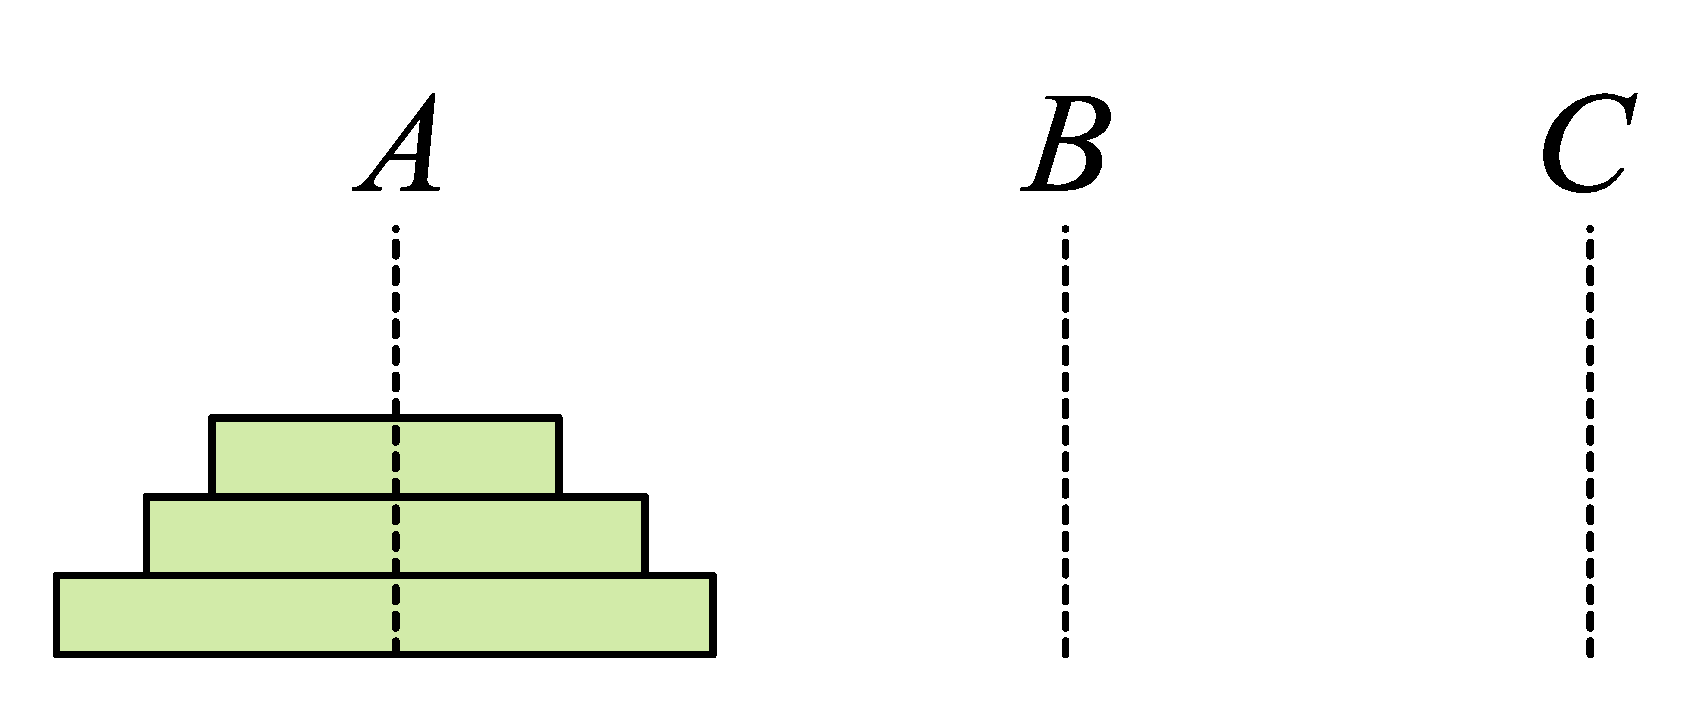
\includegraphics[width=0.35\textwidth]{images/title/汉诺塔问题.pdf}
		\caption{汉诺塔问题}
		\label{fig:汉诺塔问题}
	\end{figure}

	\solution
	\\

	该问题即为著名的汉诺塔问题, 递归式的求解算法描述为: 先将$A$上面的$n-1$个盘子移到$B$, 再将$A$中最下边的盘子移动到$C$, 再将$B$中的$n-1$个盘子移动到$C$上即可. 伪码描述为算法\ref{alg:汉诺塔算法}:
	\begin{algorithm}[H]
		\begin{algorithmic}[1]
		\Require{$n$个盘子从上往下、从小到大放在$A$柱}
		\Ensure{将$A$柱的圆盘移到$C$柱上}
		\If{$n$ == 1}
			\State move $(A, C)$;
		\Else
			\State $\textbf{Hanoi}(A, B, n-1)$;
			\State move $(A, C)$;
			\State $\textbf{Hanoi}(B, C, n-1)$;
		\EndIf
		\State \textbf{end \{Hanoi\}}
		\end{algorithmic}
		\caption{汉诺塔问题的递归算法$\textbf{Hanoi}(A, C, n)$}
		\label{alg:汉诺塔算法}
	\end{algorithm}
	易知$T(1)=1$, 根据上述伪码可知时间复杂度有递推方程
	\begin{align}
		T(n) = 2T(n-1)+1
	\end{align}
	于是通过递推得到
	\begin{align}
		T\left( n \right) &=2T\left( n-1 \right) +1=2\left( 2T\left( n-2 \right) +1 \right) +1 \notag
		\\
		&=2^2T\left( n-2 \right) +1+2^1 \notag
		\\
		&=2^3T\left( n-3 \right) +1+2^1+2^2 \notag
		\\
		&=2^{n-1}T\left( 1 \right) +1+2+\cdots +2^{n-2} \notag
		\\
		&=2^n-1 \notag
	\end{align}
	于是$T(n)=\Theta \left(2^n\right)$. 而且可以证明的是, 汉诺塔问题不存在多项式时间算法, 因此是一个难解的问题.
\end{homeworkProblem}

\pagebreak


\begin{homeworkProblem}

	给定含有$n$个不同数的数组$L=\left\{ x_1,x_2,\cdots, x_n \right\}$, 若$L$中存在$x_i$, 使得$x_1<x_2<\cdots<x_{i-1}<x_i>x_{i+1}>\cdots >x_n$, 则称$L$是单峰的, 并称$x_i$是$L$的峰顶. 假设$L$是单峰的, 设计一个优于$O(n)$的算法找到$L$的峰顶.
	\\

	\solution
	\\

	\textbf{算法思路描述:} 对区间$[0,n-1]$进行二分, 不妨设中点为mid$=\left\lfloor (n-1)/2\right\rfloor $. 
	
	观察中点的左右邻点: 
	\begin{itemize}
		\item \textbf{case1:} 若$L\left[ \mathrm{mid}-1 \right] <L\left[ \mathrm{mid} \right] <L\left[ \mathrm{mid}+1 \right]$, 则显然峰顶在右半区间$[\text{mid} +  1, n - 1]$, 在该区间继续二分搜索即可;
		\item \textbf{case2:} 若$L\left[ \mathrm{mid}-1 \right] >L\left[ \mathrm{mid} \right] >L\left[ \mathrm{mid}+1 \right]$, 则显然峰顶在左半区间$[0, \text{mid} -  1]$, 在该区间继续二分搜索即可;
		\item \textbf{case2:} 若$L\left[ \mathrm{mid}-1 \right] <L\left[ \mathrm{mid} \right] >L\left[ \mathrm{mid}+1 \right]$, 则显然峰顶就是$L\left[ \mathrm{mid} \right]$, 至此搜索完毕.
	\end{itemize}
	对应的算法伪代码见如下:
	\begin{algorithm}[H]
		\begin{algorithmic}[1]
		\Require{$n$个不同数的数组$L[0,n-1]$且$L$为单峰数组}
		\Ensure{$L$的峰顶}
		\If{$n$ == 3} \Comment{因为已知$L$为单峰数组, 因此$n\geq 3$}
			\State \Return $L[1]$; \Comment{若$n=3$, 则显然$L[1]$为峰顶}
		\Else
			\State \textbf{int} low = 0, high = $n-1$;
			\While{low <= high}
				\State \textbf{int} mid = (low + high) $>>$ 1;
				\If{$L\left[ \mathrm{mid}-1 \right] <L\left[ \mathrm{mid} \right] >L\left[ \mathrm{mid}+1 \right]$}
					\State \Return $L\left[ \mathrm{mid} \right]$;
				\ElsIf{$L\left[ \mathrm{mid}-1 \right] <L\left[ \mathrm{mid} \right] <L\left[ \mathrm{mid}+1 \right]$}
					\State low = mid $+$ 1;
				\Else
					\State high = mid $-$ 1;
				\EndIf
			\EndWhile
		\EndIf
		\State \textbf{end \{peakIndex\}}
		\end{algorithmic}
		\caption{单峰数组的二分搜索算法$\textbf{peakIndex}(L)$}
		\label{alg:单峰数组的二分搜索算法}
	\end{algorithm}
	现在来分析算法的时间复杂度$T(n)$: 因为每一次二分都只需要做两次(常数次)比较, 所以$T(n)$的递归方程为$T\left( n \right) =T\left( n/2 \right) +O\left( 1 \right) $, 根据主定理($a=1,b=2,d=0$)可解得$T\left( n \right) =O\left( \log n \right) $.
\end{homeworkProblem}

\pagebreak

\begin{homeworkProblem}

	设$A$是$n$个不同元素组成且排好序的数组, 给定数$L$和$U$, $L<U$, 设计一个优于$O(n)$的算法, 找到$A$中满足$L<x<U$的所有数$x$.
	\\

	\solution 重新写!!!!
	\\

	\textbf{算法思路描述:} 我们需要分类讨论:
	\begin{itemize}
		\item 当$L>=A[n-1]$或$U<=A[0]$时, 显然数集$x=\emptyset$;
		\item 当$L<A[0]<U<A[n-1]$时, 用下述的\hyperref[alg:lowerbound算法]{\textbf{lowerbound算法}}找到数组$A$中第一个大于等于$U$的元素索引$q$, 则$x=\left\{ A\left[ 0 \right] ,A\left[ 1 \right] ,\cdots ,A\left[ q-1 \right] \right\}$; 
		\item 当$L=A[0]<U<A[n-1]$时, 则$x=\left\{ A\left[ 1 \right] ,A\left[ 2 \right] ,\cdots ,A\left[ q-1 \right] \right\}$;
		\item 当$A[0]<L<U<A[n-1]$时, 则先用\textbf{Problem 5}的\hyperref[alg:upperbound算法]{\textbf{upperbound算法}}找到数组$A$中第一个大于$L$的元素索引$p$, 再用\hyperref[alg:lowerbound算法]{\textbf{lowerbound算法}}找到数组$A$中第一个大于等于$U$的元素索引$q$, 这样就有$$x=\left\{ A\left[ p \right] ,A\left[ p+1 \right] ,\cdots ,A\left[ q-1 \right] \right\}$$
		\item 当$A\left[ 0 \right] <L<U=A\left[ n-1 \right] $时, 则用\hyperref[alg:upperbound算法]{\textbf{upperbound算法}}找到数组$A$中第一个大于$L$的元素索引$p$, 于是$x=\left\{ A\left[ p \right] ,A\left[ p+1 \right] ,\cdots ,A\left[ n-2 \right] \right\}$;
		\item 当$A\left[ 0 \right] <L<A\left[ n-1 \right] <U$时, 则用\hyperref[alg:upperbound算法]{\textbf{upperbound算法}}找到数组$A$中第一个大于$L$的元素索引$p$, 则$x=\left\{ A\left[ p \right] ,A\left[ p+1 \right] ,\cdots ,A\left[ n-1 \right] \right\}$;
	\end{itemize}
	  

	\begin{algorithm}[H]
		\begin{algorithmic}[1]
		\Require{长度为$n$的升序数组$A[0,\cdots,n - 1]$, 目标元素target}
		\Ensure{第一个大于等于target的元素下标}
		\State \textbf{int} low = 0, high = $n - 1$;
		\While{low $<=$ high}
			\State \textbf{int} mid = (low + high) $>>$ 1;
			\If{$A[\text{mid}] < \text{target}$}
				\State low = mid + 1;
			\Else
				\State high = mid $-$ 1;
			\EndIf
		\EndWhile
		\State \Return low; \Comment{返回所要求的下标}
		\State \textbf{end \{lowerbound\}}
		\end{algorithmic}
		\caption{二分查找\textbf{lowerbound}算法}
		\label{alg:lowerbound算法}
	\end{algorithm}
	此题主要在于分类讨论和第4种情况的求解, 其对应的C++程序非常简单(直接用一下STL的lower_bound和upper_bound二分查找函数即可), 故此处就不再罗列了. 而本文所构造的算法主要用到了两个二分查找的函数, 显然该算法的时间复杂度为$O(\log n)$, 是优于$O(n)$的.
\end{homeworkProblem}

\pagebreak


\begin{homeworkProblem}
	设$A=\left\{ a_1,a_2,\cdots ,a_n \right\} ,B=\left\{ b_1,b_2,\cdots ,b_m \right\}$是整数集合, 其中$m=O(\log n)$, 设计一个优于$O(nm)$的算法找出集合$C=A\cap B$.
	

	\solution

	\textbf{方法2 (排序+二分查找):} \textbf{算法思想描述:} 由于数组$B$比较短, 所以先对其进行排序, 然后遍历数组$A$的元素, 在排序后的$B$中使用二分查找来检索该元素, 若找到则放入$C$中. 算法伪码描述如下:
	\begin{algorithm}[H]
		\begin{algorithmic}[1]
		\Require{数组$A[0,\cdots,n-1],B[0,\cdots,m-1]$}
		\Ensure{数组$C$, 其中$C=A\cap B$}
		\State \textbf{vector<int>} $C$;
		\State $\textbf{sort}(B.\text{begin}(), B.\text{end}())$;  \Comment{对数组$B$进行原地排序}
		\For{$i=0$; $i<n$; $i$++}
			\State \textbf{bool} flag = $\textbf{binary_search}(B.\text{begin}(), B.\text{end}(), A[i])$;
			\If{flag == $\mathtt{true}$}
				\State $C.\textbf{push_back}(A[i])$;
			\EndIf
		\EndFor
		\State \Return $C$;
		\State \textbf{end \{Intersection\}} \Comment{算法的C++代码跟伪代码非常相似, 就不列出了}
		\end{algorithmic}
		\caption{数组交集算法\textbf{Intersection}}
		\label{alg:交集算法}
	\end{algorithm}
	现在来分析一下此方法的时空复杂度: 对$B$排序需要$O(m\log m)$的时间, 遍历+二分查找需要消耗$O(n\times \log m)$的时间, 所以总的时间复杂度为$O\left( m\log m \right) +O\left( n\log m \right) =O\left( \left( m+n \right) \log m \right) =O\left( n\log m \right) =O\left( n\log\log n \right)$; 而数组$B$排序所用到的栈空间为$O(\log m)$, 对$B$二分查找所需的栈空间为$O(\log m)$, 所以算法的空间复杂度为$O(\log m)=O(\log \log n)$.
	\newpage
\end{homeworkProblem}


\pagebreak

\begin{homeworkProblem}
	设$S$是$n$个不等的正整数的集合, $n$为偶数, 给出一个算法将$S$划分为子集$S_1$和$S_2$, 使得$\left\lvert S_1\right\rvert =\left\lvert S_2\right\rvert $且$\displaystyle \left| \sum_{x\in S_1}{x}-\sum_{x\in S_2}{x} \right|$达到最大, 即两个子集元素之和的差达到最大 (要求时间复杂度$T(n)=O(n)$).
	\\

	\solution
	\\
	
	\textbf{算法思想描述:} 先利用\textbf{PartSelect算法}选取数组$S$的第$n/2+1$小的元素, 并将该元素作为pivot并利用\textbf{Partition算法}来对数组$S$进行\textbf{一次划分}, 低区元素全部进入$S_2$, 高区元素和pivot都进入到$S_1$(由于$n$为偶数, 所以能够保证$\left| S_1 \right|=\left| S_2 \right|$), 这样就能够确保$\displaystyle \left| \sum_{x\in S_1}{x}-\sum_{x\in S_2}{x} \right|$达到最大. 
	算法伪码见如下:
	\begin{algorithm}[H]
		\begin{algorithmic}[1]
		\Require{数组$S[0,\cdots,n-1]$} \Comment{$n$为偶数, $S$的元素彼此互异都为正整数}
		\Ensure{$\displaystyle \max_{\left| S_1 \right|=\left| S_2 \right|} \left| \sum_{x\in S_1}{x}-\sum_{x\in S_2}{x} \right|$}
		\State \textbf{vector<int>} $S_1(n/2),S_2(n/2)$;
		\State \textbf{int} pivot = $\textbf{PartSelect}\left( S,0,n-1,n/2+1 \right)$; \Comment{求数组$S$第$n/2+1$小的元素, 可以认为是"中位数"}
		\State \textbf{int} low = 0, high = $n-1$; \Comment{对撞双指针做一次划分}
		\While{low < high}
			\While{low < high \&\& $S[\text{high}]$ >= pivot}
				\State high-\,-;
			\EndWhile
			\State $\textbf{swap}(S[\text{low}], S[\text{high}])$;
			\While{low < high \&\& $S[\text{low}]$ <= pivot}
				\State low++;
			\EndWhile
			\State $\textbf{swap}(S[\text{low}], S[\text{high}])$;
		\EndWhile
		\State \textbf{int} loc = low; \Comment{此时的loc即为pivot所处的最终下标}
		\State \textbf{copy}($S$.begin(), $S$.begin() + loc, $S_2$.begin()); \Comment{低区进入$S_2$}
		\State \textbf{copy}($S$.begin() + loc, $S$.begin() + $(n - \text{loc})$, $S_1$.begin()); \Comment{高区和pivot进入$S_1$}
		\State \Return $S_1,S_2$; \Comment{注意到$\text{loc}$其实就是$n/2$, 因此$n - \text{loc}$即为$n/2$}
		\State \Return $\textbf{accumulate}(S_1.\text{begin}(), S_1.\text{end}(), 0)-\textbf{accumulate}(S_2.\text{begin}(), S_2.\text{end}(), 0)$;
		\State \textbf{end \{MaxSubtract\}}
		\end{algorithmic}
		\caption{最大化子集和差算法\textbf{MaxSubtract}}
		\label{alg:最大化子集和差算法}
	\end{algorithm}

	现在来分析一下算法的时间复杂度: 调用\textbf{PartSelect算法}最坏需要$O(n)$的时间, \textbf{Partition算法}(核心是对撞双指针)需要$O(n)$的时间, 所以总的时间复杂度为$T(n)=O(n)+O(n)=O(n)$.
\end{homeworkProblem}



\pagebreak

\begin{homeworkProblem}
	考虑第三章PPT NO.17 $\textbf{Select}(A,k)$算法: 

	(1). 如果初始元素分组$r=3$, 算法的时间复杂度如何?
	(2). 如果初始元素分组$r=7$, 算法的时间复杂度如何?


	\solution
	

	\textbf{(1)}. 若$r=3$, 既可以认为子问题的规模为$2n/3$. 求中位数的中位数所递归调用的规模为$n/3$, 一趟快排和插入排序的所需时间为$cn$. 综上, 时间复杂度的递推方程为
	\begin{align}
		T\left( n \right) =T\left( \frac{n}{3} \right) +T\left( \frac{2n}{3} \right) +cn
	\end{align}
	画出$T(n)$的递归树, 见如下图\ref{fig:递归树-1}:
	\begin{figure}[H]  % 这里记得用[H]
		\centering
		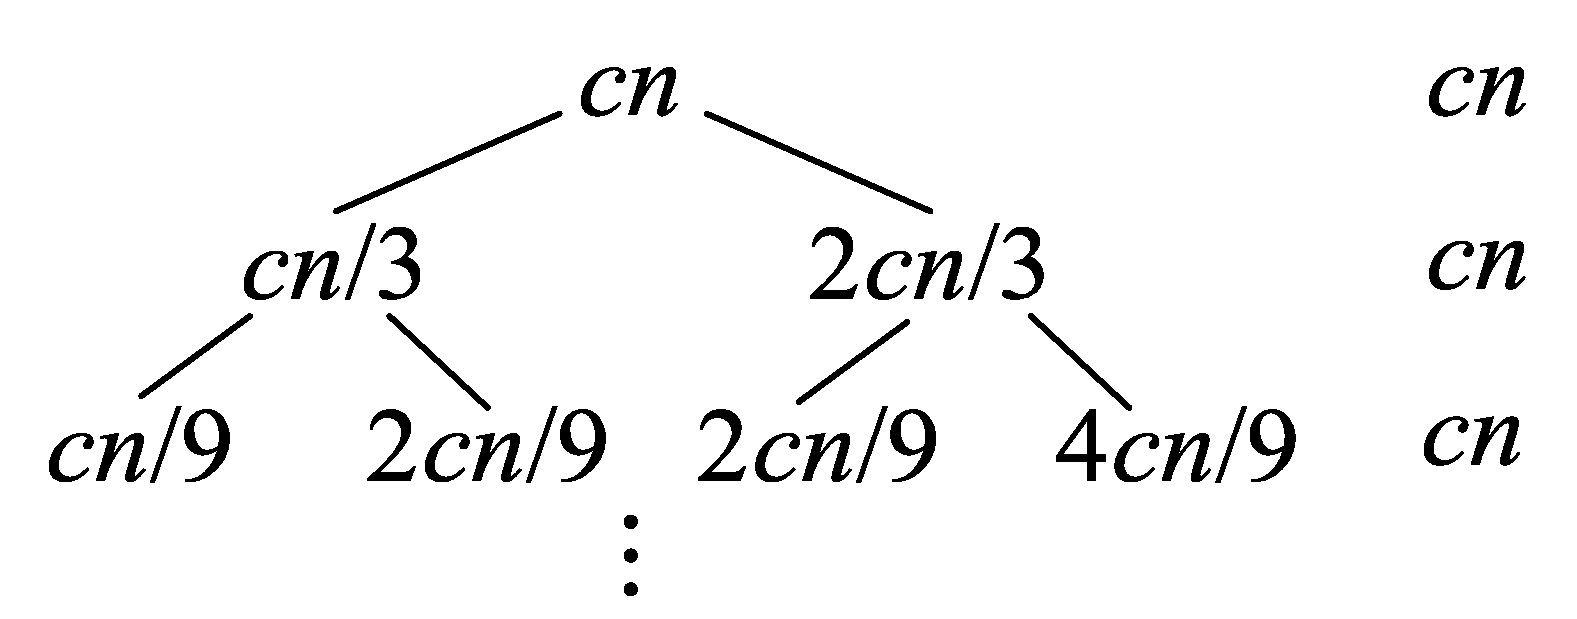
\includegraphics[width=0.4\linewidth]{images/title/递归树1.pdf}
		\caption{递归树-1}
		\label{fig:递归树-1}
	\end{figure}
	而递归树的深度为$\log n$, 而每一层的操作都是$cn$, 所以时间复杂度$T(n)=O(cn\log n)=O(n\log n)$;
	\textbf{(2)}.若$r=7$, 即可以认为子问题的规模为$5n/7$. 求中位数的中位数所递归调用的规模为$n/7$, 一趟快排和插入排序的所需时间为$cn$. 综上, 时间复杂度的递推方程为
	\begin{align}
		T\left( n \right) =T\left( \frac{n}{7} \right) +T\left( \frac{5n}{7} \right) +cn
	\end{align}
	画出$T(n)$的递归树, 见如下图\ref{fig:递归树-2}:
	\begin{figure}[H]  % 这里记得用[H]
		\centering
		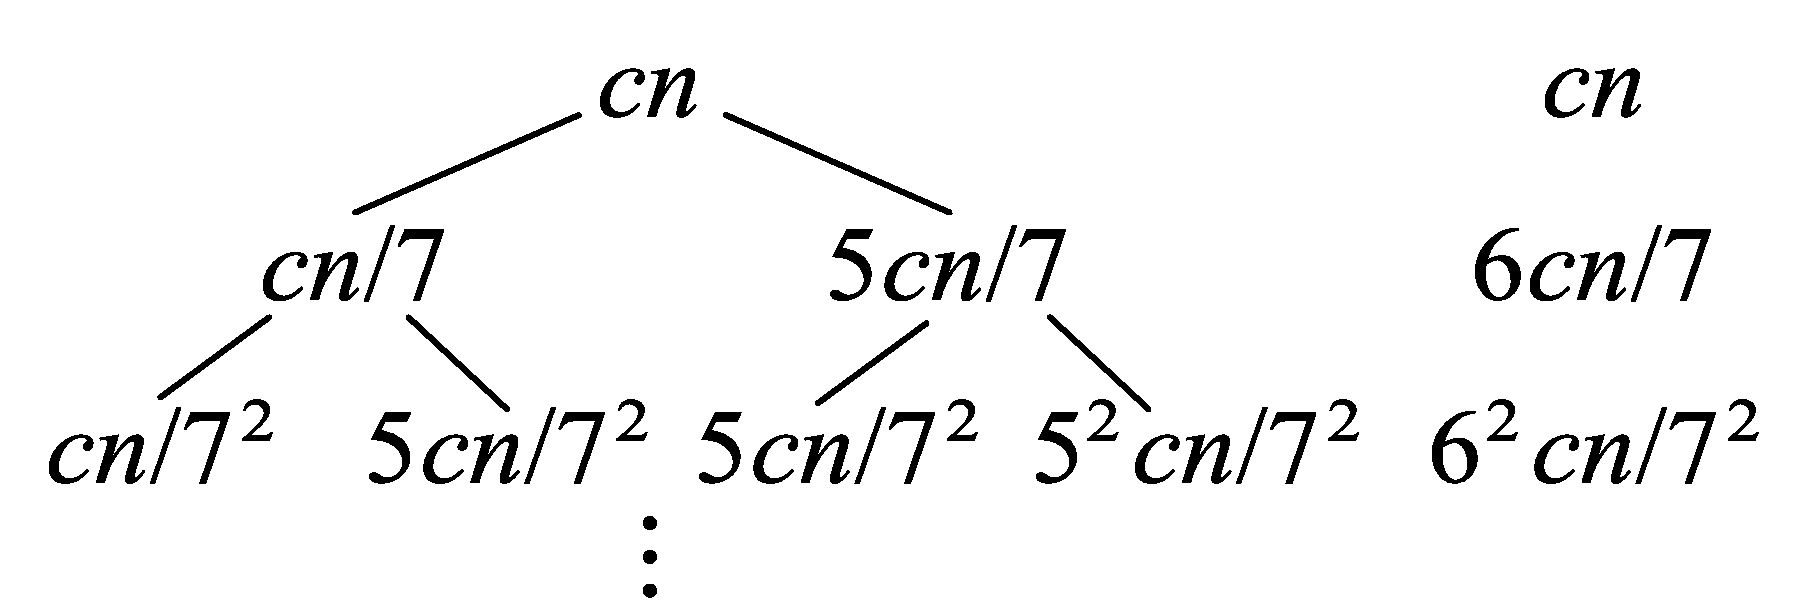
\includegraphics[width=0.4\linewidth]{images/title/递归树2.pdf}
		\caption{递归树-2}
		\label{fig:递归树-2}
	\end{figure}
	故总的时间复杂度为:
	\begin{align}
		T\left( n \right) =cn\left( 1+\frac{6}{7}+\left( \frac{6}{7} \right) ^2+\cdots \right) \le cn\cdot \frac{1}{1-\frac{6}{7}}=7cn=O\left( n \right) 
	\end{align}
\end{homeworkProblem}

\pagebreak


\begin{homeworkProblem}
	对玻璃瓶做强度试验, 设地面高度为0, 从0向上有$n$个高度, 记为$1,2,\cdots,n$, 其中任何两个高度之间的距离都相等. 如果一个玻璃瓶从高度$i$落到地上没有摔碎, 但从高度$i+1$落到地上摔碎了, 那么就将玻璃瓶的强度记为$i$.

	(1). 假设每种玻璃瓶只有1个测试样品, 设计算法来测试出每种玻璃瓶的强度. 以测试次数作为算法的时间复杂度, 估计算法的复杂度;

	(2). 假设每种玻璃瓶有足够多的相同的测试样品, 设计算法使用最少的测试次数来完成测试;

	(3). 假设每种玻璃瓶只有2个相同的测试样品, 设计次数尽可能少的算法完成测试.
	\\

	\solution
	\\

	\textbf{(1).} 顺序从下到上测试, 一次一个高度, 最坏情况下时间复杂度为$T(n)=O(n)$;

	\textbf{(2).} 因为高度越高, 玻璃瓶越容易碎, 其实可以理解为"升序数组". 因此我们可以考虑用二分法: 先在高度$n/2$测试玻璃瓶, 如果摔碎了, 则玻璃瓶的强度位于$[1,n/2-1)$(在该区间继续二分搜索即可); 若没摔碎, 则玻璃瓶的强度位于$[n/2+1,n]$(在该区间继续二分搜索即可). 显然, 该二分搜索的时间复杂度为$T(n)=O(\log n)$;
	
	\textbf{(3).} 不失一般性, 不妨设$\sqrt{n}$为整数, 则可以将$1,2,3,\cdots,n$这些$n$个高度分成$\sqrt{n}$组\footnote{如果$\sqrt{n}$不是整数, 则取$\left\lfloor \sqrt{n}\right\rfloor $个整组, 剩下的单独成一组}. 那么第$j$组($j=1,2,\cdots,\sqrt{n}$)所含有的高度有
	\begin{align}
		\left( j-1 \right) \sqrt{n}+1,\left( j-1 \right) \sqrt{n}+2,\cdots ,\left( j-1 \right) \sqrt{n}+\sqrt{n},\quad j=1,2,\cdots ,\sqrt{n}
	\end{align}

	先拿第一个瓶子测试: 从下往上, 按照每组的最大高度(即$j\sqrt{n},j=1,2,\cdots,\sqrt{n}$)进行测试. 如果前$j-1$组的测试中瓶子都没有碎, 而在第$j$组的测试中碎了, 则强度显然位于第$j$组的$\sqrt{n}$个高度中. 于是, 至多经过$\sqrt{n}$此测试, 待检查的高度范围就缩减到原来的$\frac{\sqrt{n}}{n}=\frac{1}{\sqrt{n}}$倍;

	再拿第二个瓶子测试: 在第$j$组的$\sqrt{n}$个高度中, 从下往上测试玻璃瓶的强度, 至多经过$\sqrt{n}$次测试, 就可以得到玻璃瓶的强度.

	现在来分析算法的时间复杂度: 显然第一个瓶子测验至多需要耗时$O(\sqrt{n})$, 第二个瓶子测试也至多需要耗时$O(\sqrt{n})$, 于是总的算法时间复杂度为
	\begin{align}
		T(n)=O(\sqrt{n})+O(\sqrt{n})=O(\sqrt{n})
	\end{align}
	\newpage
\end{homeworkProblem}

\pagebreak

\begin{homeworkProblem}
	\textbf{1.} 使用主定理求解以下递归方程:

	(1). $\begin{cases}
		T\left( n \right) =9T\left( n/3 \right) +n\\
		T\left( 1 \right) =1\\
	\end{cases}$;  (2). $\begin{cases}
		T\left( n \right) =5T\left( n/2 \right) +\left( n\log n \right) ^2\\
		T\left( 1 \right) =1\\
	\end{cases}$;  (3). $\begin{cases}
		T\left( n \right) =2T\left( n/2 \right) +n^2\log n\\
		T\left( 1 \right) =1\\
	\end{cases}$


	\solution
	

	\textbf{(1).} 易知$a=9,b=3,d=1,f(n)=n$, 由于$f\left( n \right) =n=O\left( n^{2-\epsilon} \right) $, 故根据主定理可知: 
	$T(n)=$
	
	$\Theta(n^2)$;

	\textbf{(2).} 易知$a=5,b=2,f(n)=n^2\log^2n=O(n^{\log_2 5-\epsilon})$, 故根据主定理可知$T(n)=\Theta \left( n^{\log_2 5} \right)$;

	\textbf{(3).} 易知$a=2,b=2,f(n)=n^2\log n=\Omega \left( n^{1+\epsilon} \right)$, 而且$$af\left( n/b \right) =2\left( n/2 \right) ^2\log \left( n/2 \right) =n^2/2\left( \log n-1 \right) \le 0.5n^2\log n\,\,\left( c=1/2<1 \right)$$
	故根据主定理可知$T(n)=\Theta(f(n))=\Theta(n^2\log n)$.

	\textbf{2.} 使用递归树求解: $\begin{cases}
		T\left( n \right) =T\left( n/2 \right) +T\left( n/4 \right) +cn\\
		T\left( 1 \right) =1\\
	\end{cases}$;
	
	\solution

	递归树见如下图\ref{fig:递归树-3}:
	\begin{figure}[H]  % 这里记得用[H]
		\centering
		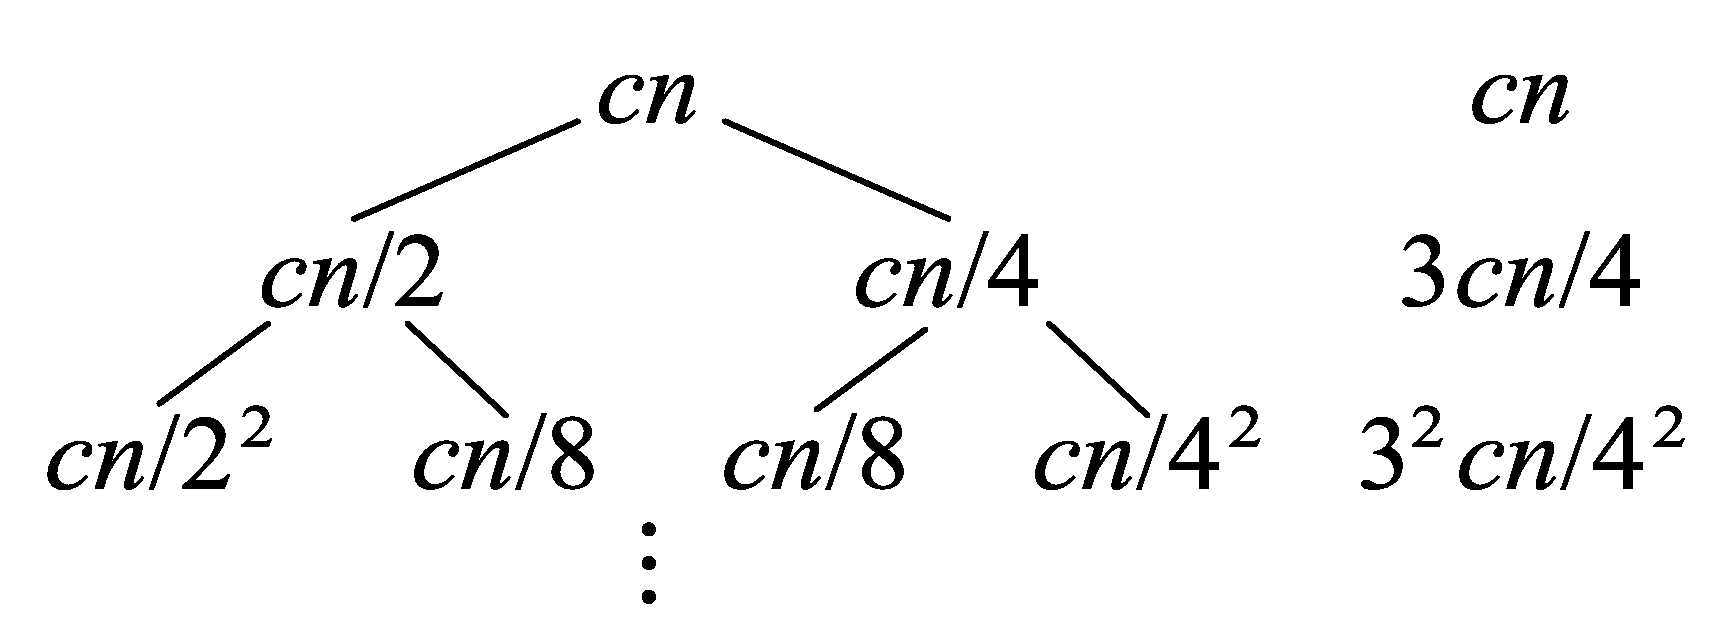
\includegraphics[width=0.4\linewidth]{images/title/递归树3.pdf}
		\caption{递归树}
		\label{fig:递归树-3}
	\end{figure}
	故总的时间复杂度为:
	\begin{align}
		T\left( n \right) =cn\left( 1+\frac{3}{4}+\left( \frac{3}{4} \right) ^2+\cdots \right) \le cn\cdot \frac{1}{1-\frac{3}{4}}=4cn=O\left( n \right) 
	\end{align}

	\textbf{3.} 使用迭代递归法求解: (1). $\begin{cases}
		T\left( n \right) =T\left( n-1 \right) +\log 3^n\\
		T\left( 1 \right) =1\\
	\end{cases}$;  (2). $\begin{cases}
		T\left( n \right) =T\left( n-1 \right) +1/n\\
		T\left( 1 \right) =1\\
	\end{cases}$.

	\solution

	\textbf{(1).} 易知
	\begin{align}
		T\left( n \right) &=T\left( n-1 \right) +\log 3^n=T\left( n-2 \right) +\log 3^{n-1}+\log 3^n
		\\
		&\cdots =T\left( 1 \right) +\log 3^2+\log 3^3+\cdots +\log 3^n
		\\
		&=1+\log \left( 3^{2+3+\cdots +n} \right) =1+\log \left( 3^{\left( n+2 \right) \left( n-1 \right) /2} \right) = \Theta \left(n^2\right)
	\end{align}

	\textbf{(2).} 易知
	\begin{align}
		T\left( n \right) &=T\left( n-1 \right) +\frac{1}{n}=T\left( n-2 \right) +\frac{1}{n-1}+\frac{1}{n}
		\\
		&\cdots =T\left( 1 \right) +\frac{1}{2}+\cdots +\frac{1}{n-1}+\frac{1}{n}=\sum_{i=1}^n{\frac{1}{i}}=\Theta \left( \gamma +\log n \right) =\Theta \left( \log n \right) 
	\end{align}
	注意, 其中我们用到了$\gamma$常数的数学结论: $\displaystyle \gamma = \lim_{n\to +\infty}\left(\sum_{i=1}^{n}\frac{1}{i}-\ln n\right)$.
\end{homeworkProblem}


% 引用文献
\bibliographystyle{unsrt}  % unsrt:根据引用顺序编号
\bibliography{refs}


\end{document}
